
\chapter{Modelo Estrutural}
\label{sec-modelo-estrutural}

O modelo conceitual estrutural visa capturar e descrever as informações (classes, associações e atributos) que o sistema deve representar para prover as funcionalidades descritas na seção anterior. A seguir, são apresentados os diagramas de classes de cada um dos subsistemas identificados no contexto deste projeto. Na seção~\ref{sec-dicionario} – Dicionário de Projeto – são apresentadas as descrições das classes, atributos e operações presentes nos diagramas apresentados nesta seção.


\section{Subsistema Core}

A Figura~\ref{figura-core-classe} apresenta o diagrama de classes do subsistema Core.

\begin{figure}[h]
  \centering
  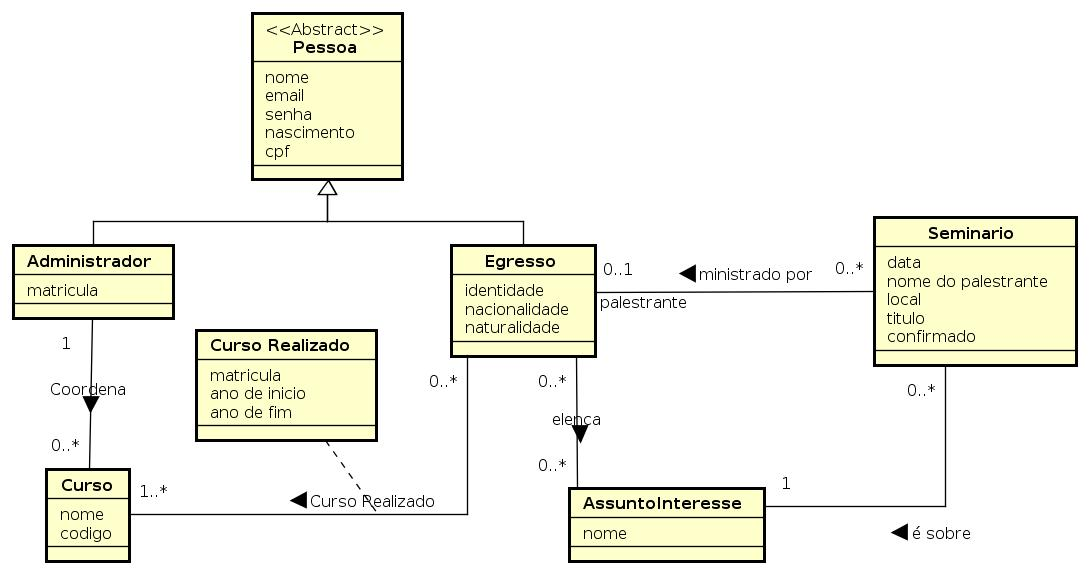
\includegraphics[width=1\textwidth]{figuras/diagrama-classe-core}
  \caption{Diagrama de Classes do Subsistema Core.}
  \label{figura-core-classe}
\end{figure} 


\newpage

\section{Subsistema Public}


A Figura~\ref{figura-public-classe} apresenta o diagrama de classes do subsistema Public.

\begin{figure}[h]
  \centering
  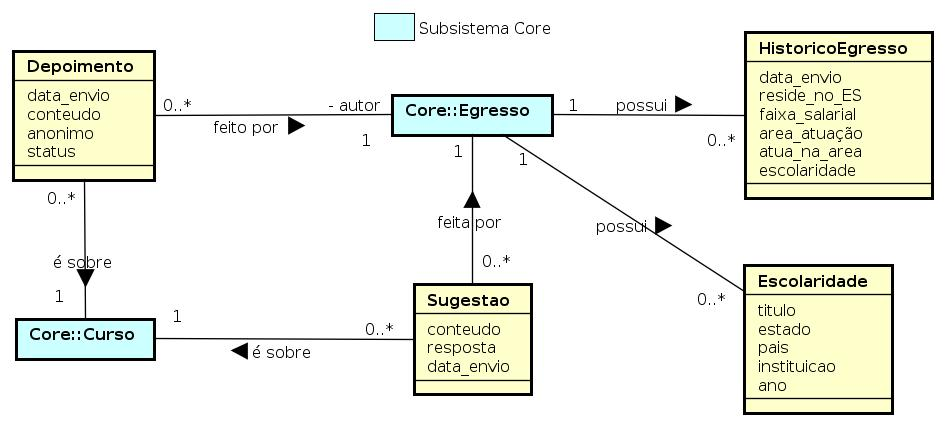
\includegraphics[width=1\textwidth]{figuras/diagrama-classe-public.jpg}
  \caption{Diagrama de Classes do Subsistema Public.}
  \label{figura-public-classe}
\end{figure} 
\newpage
